% !TEX root = ../my-thesis.tex
% \newcommand{\perr}{|\nicefrac{(\hat p -\Tilde{p})}{\Tilde{p}}|}
% \newcommand{\by}{\textbf{y}}
% \newcommand{\AIC}{\text{AIC}}
% \newcommand{\M}{\mathcal{M}}

\graphicspath{{./content/chap3_mini-batching/}}

% \setcounter{equation}{0}
% \setcounter{figure}{0}
% \setcounter{table}{0}
% % \setcounter{page}{1}
% \makeatletter % changes the catcode of @ to 11
% \renewcommand{\thetable}{S\arabic{table}}
% \renewcommand{\theequation}{S\arabic{equation}}
% \renewcommand{\thefigure}{S\arabic{figure}}
% \makeatother % changes the catcode of @ back to 12

\section{Supplementary Information}
\label{secSI:mini-batching}

We show that the loss function $L_\M(\theta)$ in the main manuscript in \cref{eq:loss_fn} is ill-behaved for models with complex dynamics when the time horizon is large. We proceed by first analysing the dynamics of models with complex dynamics showing chaotic behaviour or limit cycles, and approximate the divergence of perturbed dynamical trajectories. We then show that the divergence in dynamics translates into a loss function whose surface is rugged in most of the parameter space, and that the gradient of the loss function around the true parameters becomes exponentially steeper with time. We conclude by formally discussing how the proposed segmentation method regularizes the ill-behaviour of the loss function.

\subsection{Dynamics under perturbations}
% For the sake of clarity and without loss of generalization, we assume in this section that the map $h$ is identity function and therefore omit it.

\subsubsection{Perturbed initial conditions}
Consider the trajectory of the state variables
\begin{equation}
\begin{split}\label{eqSI:prob_statement}
        x(t) &= \M(t,p,x_0)\\
            &=\int_0^t f(s, x(s), p) ds + x_0
\end{split}
\end{equation}
and consider the perturbed trajectory 
\begin{equation}\label{eqSI:prob_statement2}
    x_{\delta x_0}(t) = \M(t, p, x_0 + \delta x_0)
\end{equation}
whose initial conditions (ICs) $x_0$ are perturbed by $\delta x_0$. Assuming that the system is chaotic and that $\delta x_0$ is small, the distance between the perturbed trajectory and the original one grows as
\begin{equation}
	\|x(t) - x_{\delta x_0}(t)\| \sim e^{\lambda t}\delta x_0
\end{equation}
where $\lambda$ is the largest Lyapunov exponent of the system \citep{strogatz2018nonlinear}.
% 
After enough time, the trajectories diverge so much that they effectively become independent samples of the phasespace: the trajectories forget their ICs, and ergodic theory ensures that the positions of $x(t)$ and $x_{\delta x_0}(t)$ are better described by a random variable $\mathcal R$ with probability density given by the density of orbits in the chaotic attractor, the so-called invariant measure of the chaotic attractor \citep{jost2005dynamical}.
% 
The distance between $x(t)$ and $x_{\delta {x_0}}(t)$ can therefore be described as 
\begin{equation}
	\|x(t) - x_{\delta x_0}(t)\| \sim \|\mathcal{R}_1 - \mathcal{R}_2 \|
\end{equation}
%
Considering the observation function $h$, it follows that
\begin{equation}\label{eqSI:divergenceTrajectoriesICs}
\begin{aligned}
	&\|h(x(t)) - h(x_{\delta x_0}(t))\| \sim \left.\frac{\partial h}{\partial x}\right|_{x(t)} e^{\lambda t}\delta x_0 \text{    for }t\ll \frac{1}{\lambda}\\
	&\|h(x(t)) - h(x_{\delta x_0}(t))\| \sim \|h\left(\mathcal{R}_1\right) - h\left(\mathcal{R}_2\right) \| \text{    for }t\gg \frac{1}{\lambda}
\end{aligned}
\end{equation}
(see \cref{figSI:perturbed_ICs} for an illustration of the divergence behaviour over time).


\subsubsection{Perturbed model parameters}
Consider now a trajectory $x_{\delta p }$ with a small perturbation of the parameters $\delta p$ .
%
From \cref{eqSI:prob_statement,eqSI:prob_statement2}, it follows that
\begin{equation}
\begin{split}
	\dot{x}_{\delta p}(t) &= f(t, x_{\delta p}(t), p + \delta p) \\
	&\sim f(t, x_{\delta p}(t), p) + \frac{\partial f(t,x_{\delta p}(t), p)}{\partial p}\delta p\\
	&\sim f(t, x(t), p) + \frac{\partial f(t,x_{\delta p}(t), p)}{\partial p}\delta p
	+\frac{\partial f(t,x(t), p)}{\partial  x(t)}\frac{\partial x(t)}{\partial p}\delta p
\end{split}
\end{equation}
which is dominated by the first term under small values of $\delta p$, and is thus subject to chaotic dynamics.
% 
Similar to a perturbation of the ICs, the small perturbation $\delta p$ generates a divergence in the dynamical trajectories that grows exponentially until they become uncorrelated.
% 
For small $\delta p$, the distance between the true and deviated trajectory can therefore be approximated as
\begin{equation}
	\begin{aligned}
		&\|x(t) - x_{\delta p}(t)\| \sim 
		\int_{0}^{t} e^{\lambda (t-s)}\|x(s) - x_{\delta p}(s)\|ds \sim e^{\lambda t} g(\delta p)
	\end{aligned}
\end{equation}
where $g(\delta p) = \|\frac{\partial f(t,x_{\delta p}(t), p)}{\partial p}+\frac{\partial f(t,x(t), p)}{\partial  x(t)}\frac{\partial x(t)}{\partial p}\|$ gives the scale of the divergence between the two trajectories as a function of $\delta p$. %This growth can be estimated as $ = \E\left[\|\frac{\partial f(t,x_{\delta p}(t), p)}{\partial p}\delta p+\frac{\partial f(t,x(t), p)}{\partial  x(t)}\frac{\partial x(t)}{\partial p}\delta p\|\right]$ which grows linearly with $\|\delta p\|$. 
% 
Similar to a perturbation of the ICs, the difference in trajectories grows to the point where the trajectories become effectively independent after a long time. Hence, it follows that
\begin{equation}\label{eqSI:divergenceTrajectoriesParameters}
\begin{aligned}
	&\|h(x(t)) - h(x_{\delta p}(t))\| \sim \left.\frac{\partial h}{\partial x}\right|_{x(t)} e^{\lambda t}g(\delta p) \text{    for }t\ll \frac{1}{\lambda}\\
	&\|h(x(t)) - h(x_{\delta p}(t))\| \sim \|h\left(\mathcal{R}_1\right) - h\left(\mathcal{R}_2\right) \| \text{    for }t\gg \frac{1}{\lambda}
\end{aligned}
\end{equation}
(see \cref{figSI:perturbed_p} for an illustration of the divergence behaviour over time).

%% 
In the following section, we call the first divergence regime the informative divergence regime, where the loss grows with the distance to the true parameters, and we call the second divergence regime the mixed divergence regime, where the loss is dominated by the random-like behaviour.
% 
Given that $\delta p$ and $\delta x_0$ behave similarly, we employ $\theta$ and $\delta \theta$ to encompass both perturbations of parameters and ICs, and denote by $g(\delta\theta)$ the function that gives the scale of the divergence in trajectories for both $g(\delta p)$ and $\|\delta x_0\|$.

%%
\subsubsection{Transition in the parameter space between the informative and the mixed regime}
% 
For a fixed time horizon $t$, and depending on the shape of the chaotic attractor, the magnitude of the perturbation determines the divergence regime. If the perturbation is small, the trajectories will be aligned, but for large perturbations they will effectively become two independent trajectories.
% The point where the transition takes place depends on the shape of the chaotic attractor and on the magnitude of the perturbation.

The transition between the two regimes can be studied by noting that the informative divergence should remain in the same order of magnitude as the mixed divergence. The reason is that the expected value of the squared divergence between two trajectories $x(t)$ and $x_{\delta \theta}(t)$ for large $t$ is
\begin{equation}\label{eqSI:ordermagnitude}
    \E\left[\|h\left(\mathcal{R}_1\right) - h\left(\mathcal{R}_2\right) \|^2\right] = 2\Var\left[h\left(\mathcal{R}\right)\right] \lesssim \max|h(\mathcal{R}) - \E\left[h(\mathcal{R})\right]|^2
\end{equation}
meaning that the expected value of the squared divergence in the mixed regime is in the same order of magnitude as the maximum distance within the phasespace. 
% 
On the other hand, the divergence of any two trajectories in the chaotic attractor cannot be larger than the maximum distance between two points in the attractor, which is itself bounded through the triangle inequality as $2\max|h(\mathcal{R}) - \E\left[h(\mathcal{R})\right]|$. 

Since the growth of the informative regime has to remain in the same order of magnitude as the mixed regime, at the regime transition we must have
\begin{equation}\label{eqSI:transitionBoundary_II}
    e^{\lambda t} g(\delta \theta) \sim \E\left[\|h\left(\mathcal{R}\right)\|\right]
\end{equation}
% 
\Cref{eqSI:transitionBoundary_II} implies that, for a given time horizon $t$, the magnitude of the critical perturbation $\delta \theta^*$ associated with the regime transition satisfies
% 
\begin{equation}\label{eqSI:transitionBoundary}
    \|\delta \theta^*\| \sim e^{-\lambda t}
\end{equation}
% \cref{eqSI:transition_boundary} implies that the radius of the ravine in which the true parameters live decreases exponentially with $\lambda t$. This implies that the minimization of \cref{eq:loss_fn}
% 
% for long time series with normal values of $t$ the ravine is so small that the initial parameters estimates will almost certainly fall outside of the ravine. Hence, gradient methods won't find it.
% In the following section, we use \cref{eqSI:transitionBoundary_II} to provide an approximation of the loss function and \cref{eqSI:transitionBoundary} to characterize the size of the region in the parameter space where the loss surface is well-behaved.

% Victor, you stopped here on the 28th of June

\subsubsection{Limit cycles}
While in the section above a chaotic system was assumed to provide an approximation for the divergence of the trajectories, a similar approximation applies for systems characterized by limit cycles.
% 
Considering a system $x(t)$ with a limit cycle characterized by the phase $\omega t$ with frequency $\omega$, i.e.~
\begin{equation}
    x(t) = \mathfrak{f}\left(\phi(t)\right)= \mathfrak{f}\left(\omega t \right) \mod 2\pi
\end{equation}
% meaning that the angle $\phi(t)$ grows with linearly with $\omega$, but since it is an angle it resets to zero after $2\pi$. 
% 
a perturbation of the parameters $\delta p$ might lead to a perturbed frequency $\delta\omega$, further leading to a difference in phases
\begin{equation}
	\delta \phi(t) = \phi(t) - \phi_{\delta\omega}(t) = \delta\omega t \mod 2\pi
\end{equation}
% 
For $t\lesssim \frac{1}{\delta \omega}$, $\delta \phi(t)$ grows linearly with $\delta \omega$, but once $t\gg \frac{1}{\delta \omega}$, the change of phase $\delta \phi(t)$ is affected by the modulo operation. As this operation is nonlinear, a small random perturbation $\delta\omega$ results in a random uniform phase over the interval $\left[0,2\phi\right]$. For a large time horizon, $x_{\delta\omega}$ is thus uniformly spread over the circular line given by the phasespace of the dynamical system. 
% 
% This can in turn be used to compute the variance of $h(\mathcal{R})$
% 
Hence, the approximation in \cref{eqSI:divergenceTrajectoriesParameters} applies for cyclic dynamics, except that the initial divergence is linear rather than exponential, and that in contrast to \cref{eqSI:divergenceTrajectoriesICs}, a change affecting the initial position will not grow over time.

\subsection{Consequences for the shape of the loss surface}

The approximation of the divergence of trajectories in \cref{eqSI:divergenceTrajectoriesICs,eqSI:divergenceTrajectoriesParameters}, together with the transition boundary determined by \cref{eqSI:transitionBoundary}, can be used to characterize the surface associated with the loss function.

%%
Omitting the term corresponding to the priors and the variance--covariance matrix $\Sigma_y$ for simplicity, the loss function presented in the main text is expressed as 
\begin{equation}
\begin{split}
	L_{\M}(\theta) &= \frac{1}{K} \sum_{k=1}^{K} ||y_{k} - h(\M(t_k,\theta))||^2\\
	                &= \frac{1}{K} \sum_{k=1}^{K} ||h(\Tilde x(t_k)) + \epsilon(t_k) - h(\M(t_k,\theta))||^2
\end{split}
\end{equation}
where the parameter vector $\theta$ is decomposed into the model parameter vector $p$ and the ICs $x_0$, $y_k$ correspond to the observations, $\Tilde x$ corresponds to the true trajectory and $\epsilon(t)$ is the observational noise. As the noise is independent of the dynamics, it is uncorrelated with $h(\Tilde x(t_k)) - \M(t_k,\theta)$, meaning that the loss can be split in expectation
\begin{equation}\label{eqSI:split_loss}
		\E\left[ L_{\M}(\theta) \right] = \frac{1}{K} \sum_{k=1}^{K} ||h(\Tilde x(t_k)) - h(\M(t_k,\theta))||^2 + \Var\left[\epsilon\right]
\end{equation}
%
where the noise term $\left(\Var\left[\epsilon\right]\right)$ is independent from the parameters $\theta$.
Assuming that $\theta = \Tilde \theta + \delta\theta$, where $\Tilde \theta$ correspond to the true parameters and ICs, every term in the sum corresponds to a squared distance between the true trajectory $\tilde x(t)$ and a perturbed trajectory $\tilde x_{\delta \theta}(t)$. Using \cref{eqSI:divergenceTrajectoriesICs,eqSI:divergenceTrajectoriesParameters,eqSI:ordermagnitude,eqSI:transitionBoundary_II} we obtain the loss function approximation
\begin{equation}\label{eqSI:lossApprox}
	L_\M(\theta) \sim \sum_{k=1}^{\min \{ K, K^*\}} e^{2\lambda t_k} g^2(\delta \theta) +
	\sum_{k=\min \{ K, K^*\} + 1}^{K} \Var \left[h(\mathcal{R})\right] +  \Var\left[\epsilon\right]
\end{equation}
% 
where $K^*$ is the observation index corresponding to the time horizon $t_{K^*}$, where the transition between the informative and the mixed regime happens for the perturbation $\delta \theta$, obtained from \cref{eqSI:transitionBoundary}.

%%
The distribution of the observation times and the magnitude of the perturbation $\delta \theta$ determine whether the loss is dominated by the informative or by the mixed divergence regime. 
% 
For a fixed perturbation $\delta \theta$, assuming that the observations $y_{k}$ are uniformly distributed over the time interval $\left[0, t \right]$, \cref{eqSI:transitionBoundary} yields for $t \ll \frac{\log(|\delta\theta|)}{\lambda}$ that the loss $L_\M$ is dominated by the informative divergence regime, whereas if $t  \gg \frac{\log(|\delta\theta|)}{\lambda}$ the loss is dominated by the mixed divergences. 
% 
In the region where the loss is dominated by mixed divergences, the loss $L_\M$ has an expected value of order $\mathcal{O}\left(\Var\left[h(\mathcal{R})\right] + \Var\left[\epsilon\right]\right)$ and does not grow monotonically with $\delta \theta$. It corresponds to a "random-like" surface populated with local minima, and is consequently characterized by an uninformative gradient preventing local optimizers from converging to the true parameters $\Tilde \theta$ (see \cref{fig:training_on_mini-batches}B, orange dashed curve).
% 
On the other hand, in the region where the divergence in trajectories belongs to the informative regime, the loss is convex and grows with $\delta \theta$. Its associated gradient $\nabla_\theta L_\M(\theta) \sim \sum_{k=1}^{K} e^{2\lambda t_k} \nabla_\theta g^2(\delta \theta)$ consequently contains relevant information for the use of variational optimizers, but the loss surface becomes exponentially steeper as the time horizon increases.
%%
As shown by the green dotted curve in \cref{fig:training_on_mini-batches}B, this large gradient in the vicinity of the optimal parameters is likely to lead gradient-based optimizers to overshoot and not converge to the true parameters $\Tilde \theta$.
% 
\cref{eqSI:transitionBoundary} further indicates that the volume of the region in the parameter space where the loss is informative shrinks exponentially as the time horizon increases, implying that for large time horizons, the uninformative region is predominant.

\subsection{Regularizing the loss surface with segments}
% 
To prevent the situation with a mixed divergence regime and to decrease the gradient in a vicinity of the true parameters, we reformulate the loss function as the average of loss functions defined over segments of short time horizons. In the following section, we compare the properties of the naive loss function $L_\M$ in \cref{eqSI:split_loss} with the segmented loss function $L^\star_\M$ proposed in \cref{eq:ML-framework} in the main manuscript, and further discuss the limitations of the method in the presence of noise.

Omitting the term corresponding to the priors and ICs and the noise shape $\Sigma_y$, and assuming a single time series for simplicity, 
% and assuming that the time steps are regularly spaced for simplicity, i.e. $t_{k+1} - t_k = T$, 
the segmented loss function presented in the main text can be expressed as
\begin{equation}\label{eqSI:mini-batch_loss_fn}
        L_\M^\star(\theta) = \frac{1}{M} \sum_{m=0}^{M-1} \frac{1}{K} \sum_{k=1}^{K^{(m)}} \|y_{k + m K/M } - h\left(\M(t_{k + m K/M}, p, x_{0}^{(m)})\right)\|^2
\end{equation}
%
where $M$ is the number of segments, $x_0^{(m)}$ corresponds to the ICs for segment $m$ inferred at time $t_{m K/M}$, and
$K^{(m)} = \begin{cases} K / M + 1 &\quad \colon m < M \\ 
                    K / M &\quad \colon m = M
        \end{cases}$ is the number of data points in the $m$th segment.
%
The loss function can be split in expectation as
\begin{equation}\label{eqSI:split_mini-batch_loss}
		\E \left[L_{\M}^{\star}(\theta) \right] = \frac{1}{M} \sum_{m=0}^{M-1} \frac{1}{K} \sum_{k=1}^{K^{(m)}} \| h(\Tilde x(t_{k + m K/M})) - \M(t_{k + m K/M},p, x_0^{(m)})\|^2 + \Var\left[\epsilon\right]
\end{equation}
% 
Assuming that $x_0^{(m)} = \Tilde x (t_{m K/M}) + \delta x_0^{(m)} $ when $\delta x_0^{(m)}$ is small, and assuming that the observation times are regularly spaced so that $t_{k+1} - t_{k} = \Delta t$, the time length of simulated trajectories (i.e. the time elapsed between the time when the perturbation is applied and the end time of the simulated trajectory) is divided by the number of segments, in comparison to the time length of the simulated trajectory in \cref{eqSI:split_loss}  ($t = t_{K/M + 1} - t_{0} = K/M \Delta t$ in \cref{eqSI:split_mini-batch_loss}, in comparison to $t = K \Delta t$ in \cref{eqSI:split_loss}).
% 
Further assuming that $K \Delta t >> \frac{\log(|\delta \theta|)}{\lambda}$ and choosing the number of segments $M$ so that $K / M \Delta t << \frac{\log(|\delta \theta|)}{\lambda}$, we apply the approximation \cref{eqSI:lossApprox}, which leads to
\begin{equation}\label{eqSI:comparision_losses}
	\begin{aligned}
		&L_{\M}(\theta) \sim \Var\left[\epsilon\right] + 
		\Var\left[ h\left(\mathcal{R}\right) \right]\\
		&L_{\M}^{\star}(\theta) \sim \Var\left[\epsilon\right] + 
		g^2(\delta \theta) \sum_{m=0}^{M-1} e^{2\lambda (K / M \Delta t)}
	\end{aligned}
\end{equation}
While $L_{\M}$ is dominated by the mixed regime, $L_\M^\star$ is dominated by the informative regime because the simulation time remains small, permitting the successful use of variational optimizers.

%%
The number of segments $M$ should be determined by considering the dynamical behaviour of the system and the level of noise in the observation, because a large number of segments $M$ smooths out the loss surface but also entails more sensitivity to the level of noise. Indeed, in $L_\M(\theta)^\star$ the relative effect of the second term corresponding to the observational noise $\epsilon$ increases when the number of segments $M$ increases.
%
The value of $M$ should therefore be chosen wisely to balance the benefits of segments, i.e. widening the region of the parameter space where $L_\M$ is well behaved and reducing the overshooting problem, and their cons, i.e. their tendency to increase the importance of noise. 

\section{Three-compartment food-web models}
\label{secSI:models}
\subsection{Reference food-web model}
We used the three-species chaotic food-web model from \citep{Hastings1991}, formulated as
\begin{equation}
    \begin{aligned}
        \tfrac{d}{dt} R &= R ( 1 - R ) - x_C y_C \frac{CR}{R + R_0}\\
        \tfrac{d}{dt} C &= x_C C \left[ -1 + x_C \frac{R}{R + R_0} \right] - x_P y_P \frac{PC}{C + C_0}\\
        \tfrac{d}{dt} P &= x_P P \left[ -1 + y_P \frac{C}{C+C_0} \right],
    \end{aligned}
\end{equation}
with the biologically realistic parameter values $x_C = 0.4$, $0.071 \leq x_P \leq 0.225 $, $y_C = 2.01$, $y_P = 5$, $R_0 = 0.16129$, and $C_0 = 0.5$ \citep{McCann1994}. The dynamics of the system are chaotic for this set of parameter values.

\subsection{Omnivory variant food-web model}
We used the three-species food-web model from \citep{McCann1997}, formulated as
\begin{equation}
    \begin{aligned}
        \tfrac{d}{dt} R &= R ( 1 - R ) - x_C x_C \frac{CR}{R + R_0} - \omega x_P y_{PR} \frac{PR}{R_{02} + (1-\omega)C + \omega R}\\
        \tfrac{d}{dt} C &= x_C C \left[ -1 + x_C \frac{R}{R + R_0} \right] - (1 - \omega) x_P y_{PC} \frac{PC}{\omega R +(1-\omega)C + C_0}\\
        \tfrac{d}{dt} P &= x_P P \Big[ -1 + (1 - \omega)x_P y_{PC} \frac{C}{\omega R + (1-\omega)C+C_0} \\
        &\qquad + \omega x_P y_{PR}\frac{R}{\omega R + (1-\omega)C + R_{02}} \Big]
    \end{aligned}
\end{equation}
with the biologically realistic parameter values $x_C = 0.4$, $ x_P = 0.08 $, $y_C = 2.009$, $y_{PR} = 2$, $y_{PC} = 5$, $R_0 = 0.16129$, $C_0 = 0.5$, and $0 \leq \omega \leq 0.5$.
% 
For this set of parameter values, the dynamics of the system are chaotic for $\omega \lesssim 0.20$, consist of a limit cycle for $0.20 \lesssim \omega \lesssim 0.35$, and consist of dampened oscillations for $ 0.35 \lesssim \omega$.

% \printbibliography[heading=subbibliography]

\section{Supplementary Figures}
% \begin{figure}[ht]
%     \centering
%     \includegraphics[width=0.8\textwidth]{figures/ill_conditioning_training_epochs.pdf}
%     \caption{Ill conditioning of $L_\M(\theta)$ leads to jumps cause by the very large gradient in a neighborhood of the true parameter.}
%     \label{ill_conditioning_training_epochs}
% \end{figure}
\begin{figure}[ht]
    \centering
    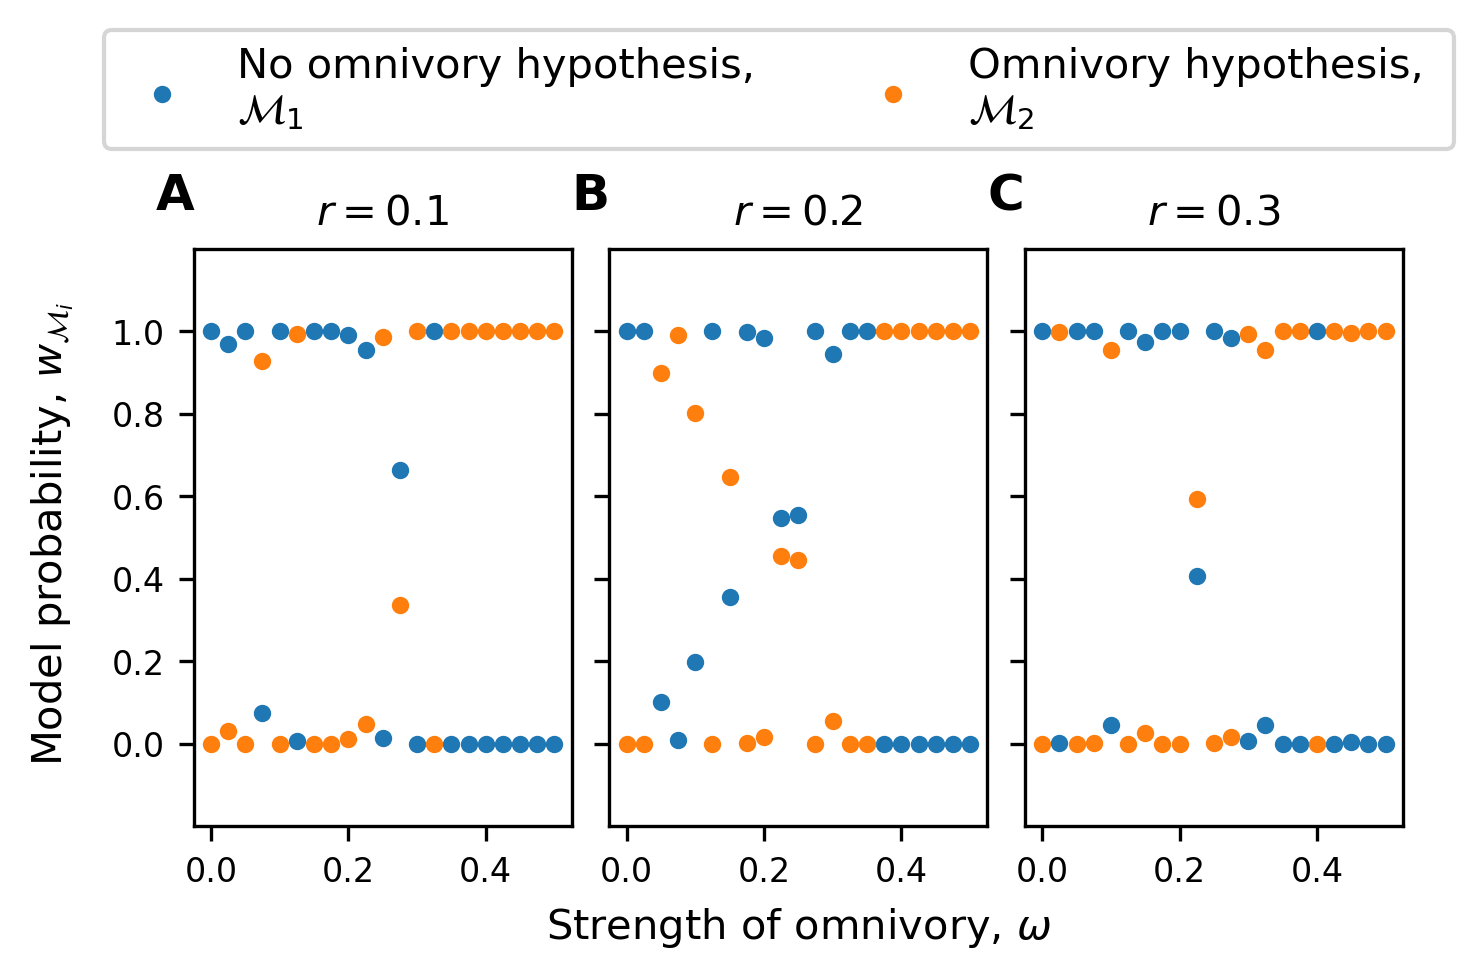
\includegraphics[]{figures/SI/figure5_2sp.png}
    \caption{\textbf{Performance of the ML framework in supporting the predator omnivory hypothesis in a food web for the partial observation setting}. 
    % 
    In \textbf{A},  \textbf{B} and \textbf{C} where $r = 0.1, 0.2 ,0.3$, the lack of data prevents the correct estimation of the omnivory variant model parameters, leading model $\M_1$ to be supported for a wider range of $\omega$ in contrast to the complete observation setting (\cref{fig:AIC_likelihood_comparision_3-compartments-model}A).}
    \label{figSI:model_selection_1sp}
\end{figure}

\FloatBarrier

\begin{figure}[ht]
    \centering
    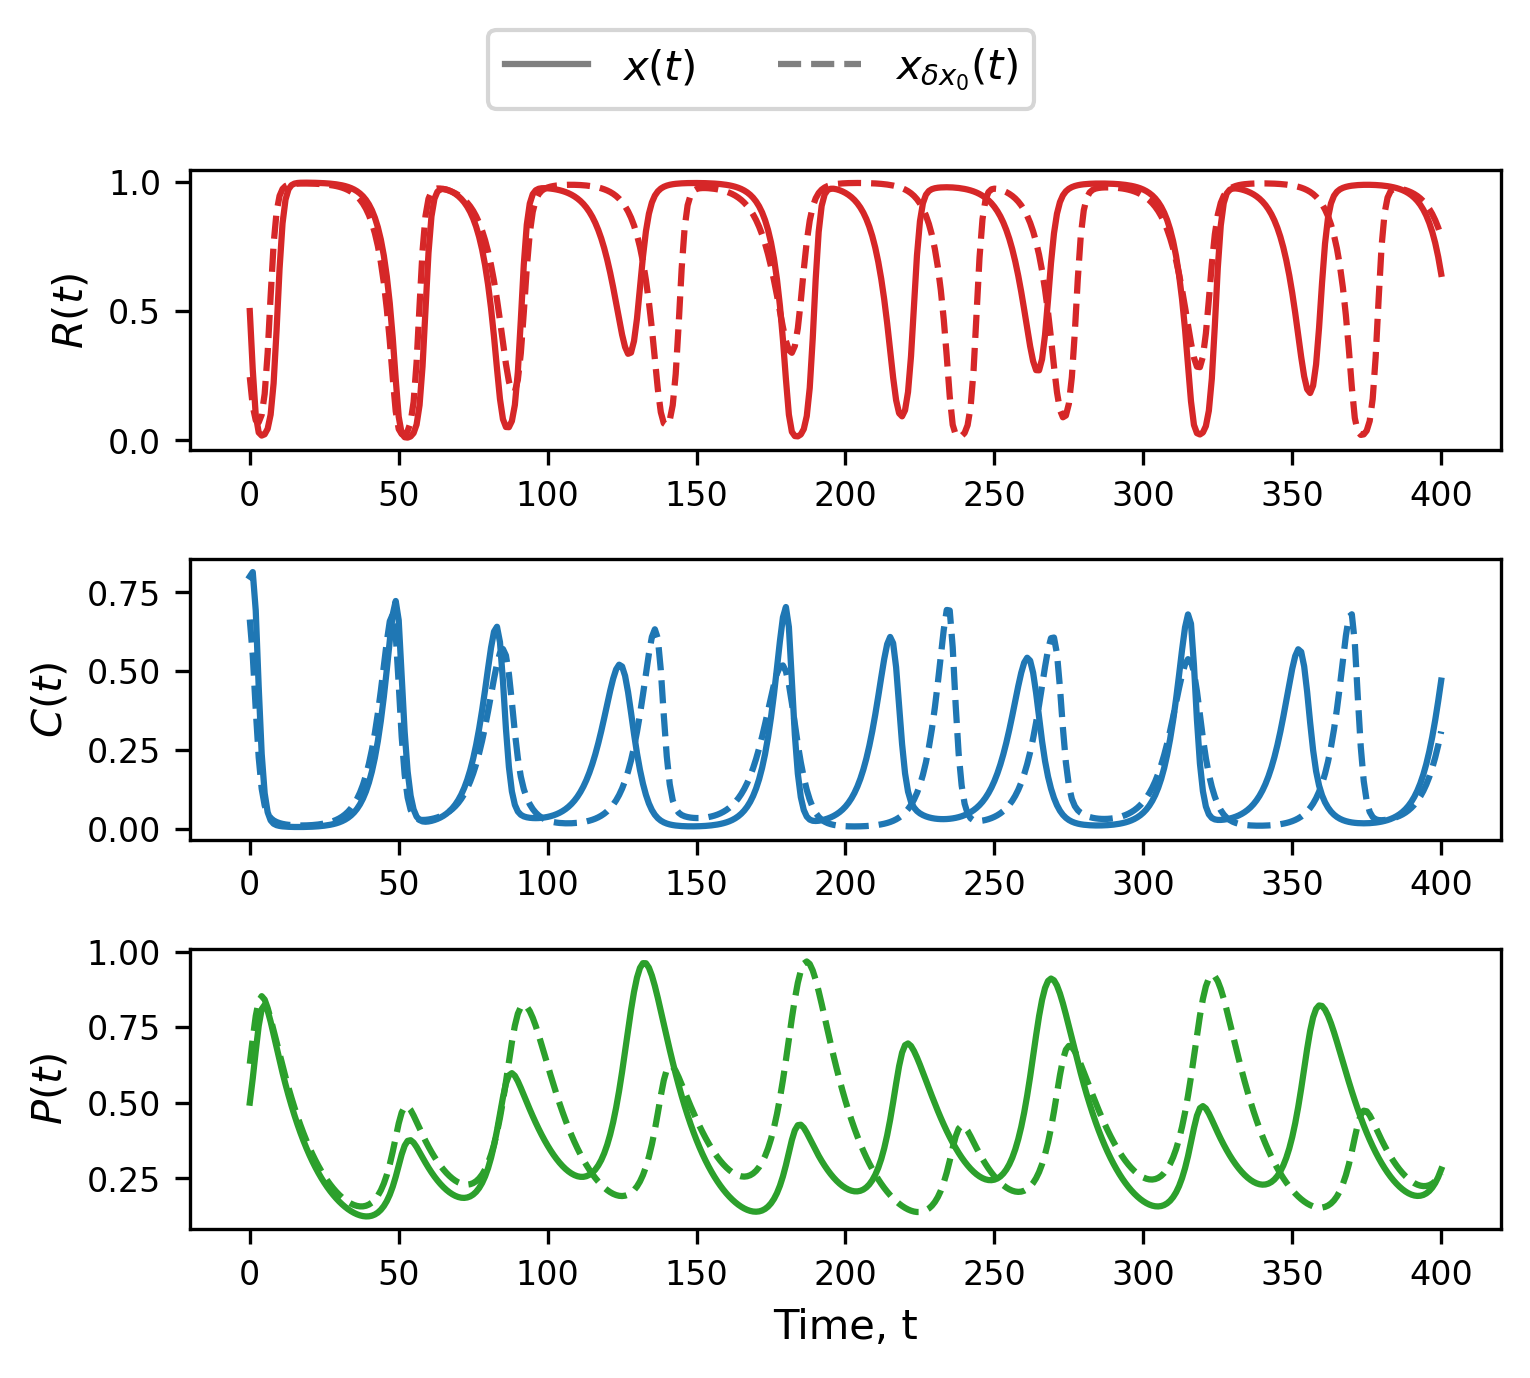
\includegraphics[]{figures/SI/perturbed_ICs.png}
    \caption{\textbf{Divergence between the trajectory $x(t)$ and a perturbed trajectory $x_{\delta x_0}(t)$, obtained from the reference food-web model from \cite{Hastings1991} and detailed in \cref{secSI:models}}. For $t \lesssim 100$, $x(t)$ and $x_{\delta x_0}(t)$ are correlated and the divergence regime is informative, but for $t \gtrsim 100$ the trajectories become essentially uncorrelated, corresponding to the mixed divergence regime.}
    \label{figSI:perturbed_ICs}
\end{figure}

\FloatBarrier

\begin{figure}[ht]
    \centering
    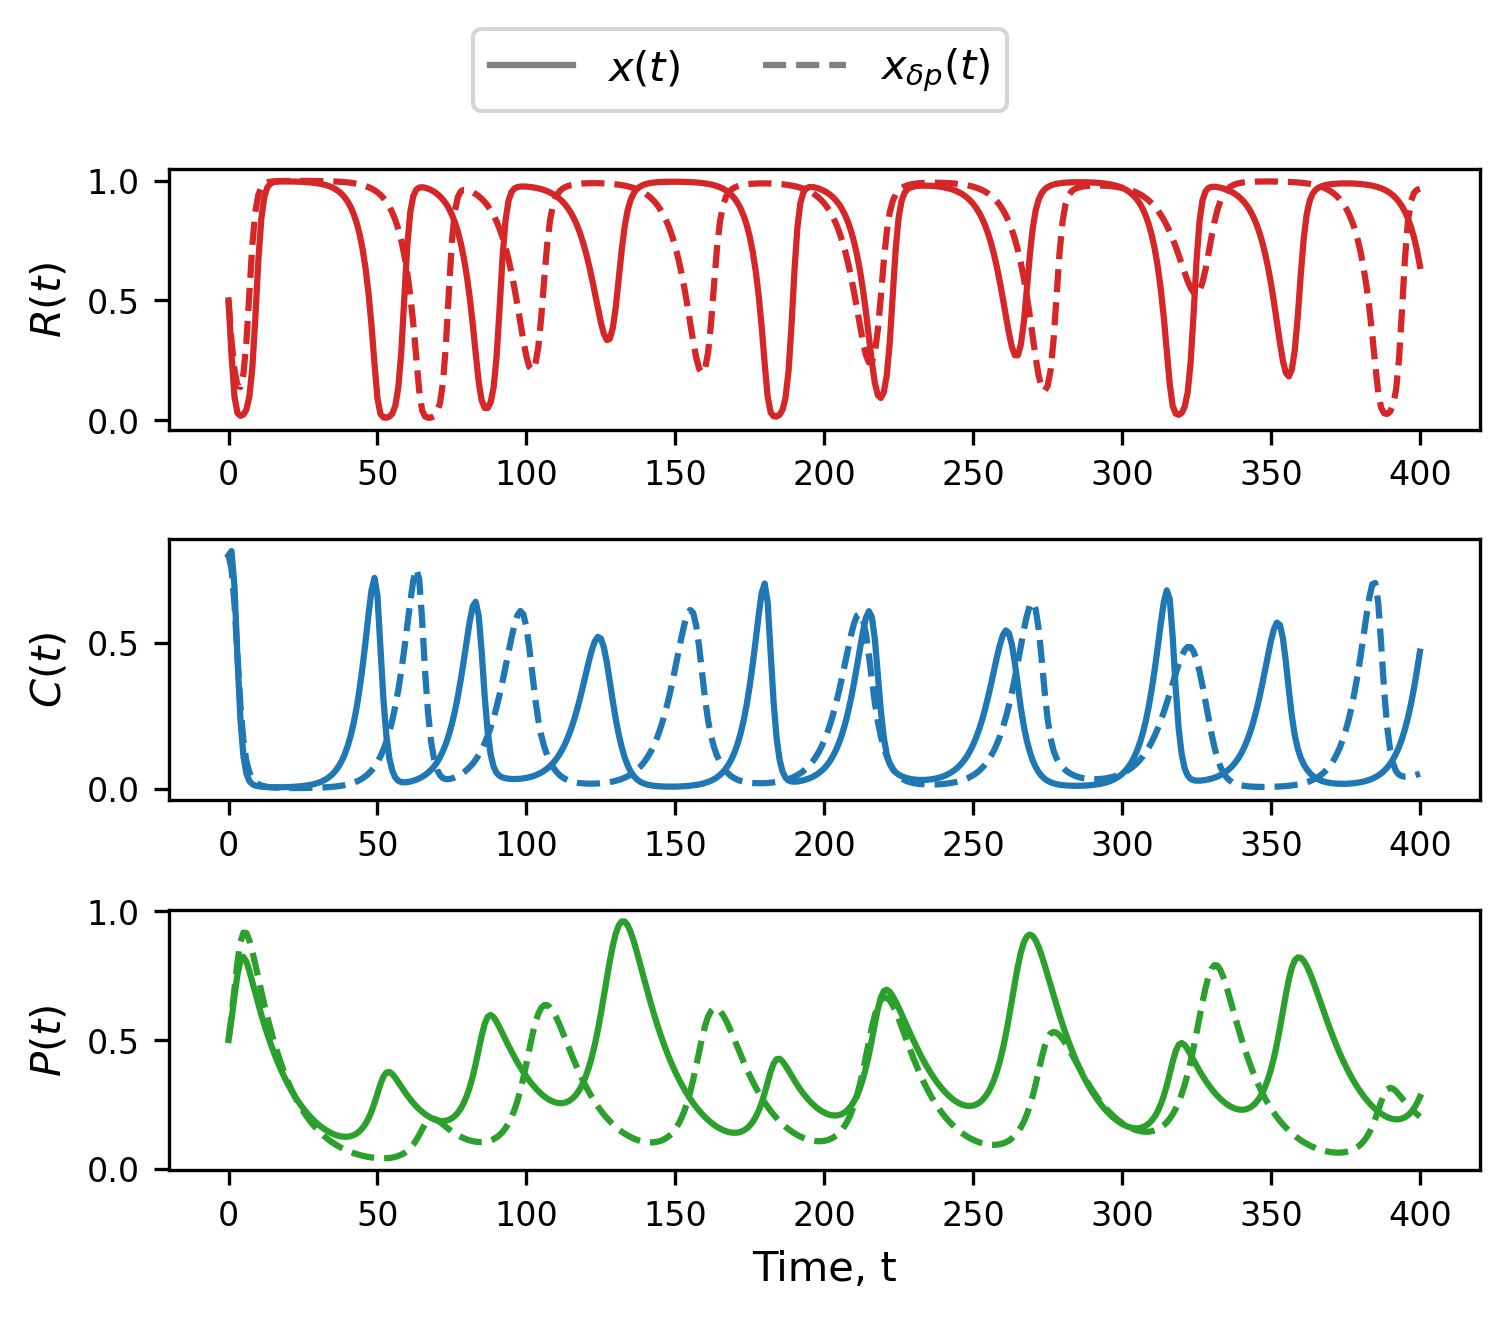
\includegraphics[]{figures/SI/perturbed_p.png}
    \caption{\textbf{Divergence between the trajectory $x(t)$ and a perturbed trajectory $x_{\delta p}(t)$, obtained from the reference food-web model from \cite{Hastings1991} and detailed in \cref{secSI:models}}. For $t \lesssim 40$, $x(t)$ and $x_{\delta p}(t)$ are correlated and the divergence regime is informative, but for $t \gtrsim 40$ the trajectories become essentially uncorrelated, corresponding to the mixed divergence regime. }
    \label{figSI:perturbed_p}
\end{figure}

\FloatBarrier

\section{Supplementary Tables}

\begin{table}[ht]
  \centering
  % \resizebox{\textwidth}{!}{%
  \resizebox{\textwidth}{!}{
    \begin{tabular}{|c|c|c|c|}
    \hline 
    Setting & Median simulation time & Mean simulation time & Std. simulation time\\
    \hline
    Complete observations & 35.9977436 & 39.5980174 & 20.5789433\\
    Partial observations & 34.1293998 & 39.1896534 & 21.8191709\\
    \hline
    \end{tabular}
  }
  \caption{\textbf{Simulation time for the complete and partial observation settings.}}
\label{tableSI:simul_time}
\end{table}

